\section{Modello Concettuale}

\subsection{Analisi dei Requisiti}

In questa sezione si analizza la richiesta del cliente, con lo scopo di definire le funzionalità che la base di dati deve soddisfare. Individueremo le entità e le associazioni del mini-word, per rappresentare in modo esaustivo e chiaro il dominio del problema. 

\begin{displayquote}\textit{
Si sviluppi un sistema informativo, composto da una base di dati relazionale e da un applicativo Java dotato di GUI (Swing o JavaFX), per la gestione del personale di un’azienda. L’azienda possiede un certo numero di impiegati, raggruppabili in 4 categorie:
\begin{itemize}
       \item Dipendente Junior : colui che lavora da meno di tre anni \mbox{nell'Azienda.}
      \item Dipendente Middle : colui che lavora da più di tre anni \mbox{nell'Azienda.} ma meno di sette.
      \item Dipendente Senior : colui che lavora da più di sette anni \mbox{nell'Azienda.}
      \item Dirigenti: la classe dirigente non ha obblighi temporali di servizio. Chiunque può diventare dirigente, se mostra di averne \mbox{le capacità.}
\end{itemize}
I passaggi di ruolo avvengono per anzianità di servizio.
}\end{displayquote}

L'incipit della richiesta è chiara : fornire una base di Dati per la Gestione del personale di un Azienda. Le Entità principali da rappresentare nel nostro mini-word sono le seguenti :  
L'Impiegato e le sue specializzazioni, in particolare, le entità Junior, Middle e Senior. 
La prima nota che risalta dalla richiesta del cliente è quella di dividere la tipologia di Impiegato per anni di appartenenza all'azienda specificando che gli scatti possibili di carriera sono svincolati dalle competenze effettive dell'impiegato e sono sanciti solamente dagli anni di lavoro. L'entità Dirigente fa eccezione da tali specializzazioni in quanto il suo ruolo non dipende dal tempo di appartenenza all'Azienda bensì dalle capacità ben specifiche.


\begin{displayquote}\textit{
 È necessario tracciare tutti gli scatti di carriera per ogni dipendente.
}\end{displayquote}
La richiesta è modellabile con una classe Storico in cui salvare ogni scatto di carriera per ogni impiegato, la data e il passaggio di ruolo; Oltre alla rappresentazione degli scatti di carriera per le specializzazioni junior, middle e Senior, bisogna considerare anche gli scatti Dirigenziali e, siccome la richiesta non è specifica a riguardo, consideriamo che un Impiegato può avere più scatti Dirigenziali.

\begin{displayquote}
\newpage
\textit{
Nell’azienda vengono gestiti laboratori e progetti. Un laboratorio ha una particolare topic di cui si occupa, un certo numero di afferenti ed un responsabile scientifico che è un dipendente senior.
}\end{displayquote}

Abbiamo la presentazione di due nuove Entità del mini-word : Laboratorio e Progetto.
L'attenzione è focalizzata sull'Entità Laboratorio, ad esso afferiscono gli Impiegati, ciò suggerisce l'associazione fra le due entità e si suppone che un impiegato può afferire a più laboratori; E' specificato anche che oltre gli afferenti, un laboratorio ha un responsabile scientifico il quale è Senior. Siccome la richiesta non è specifica a riguardo, si considera il responsabile scientifico univoco per ogni laboratorio, in quanto è specializzato nel topic di quest'utlimo.

\begin{displayquote}\textit{
Un progetto è identificato da un CUP (codice unico progetto) e da un nome (unico nel sistema). Ogni progetto ha un referente scientifico, il quale deve essere un dipendente senior dell’ente, ed un responsabile che è uno dei dirigenti.
}\end{displayquote}

Il focus è spostato sulla nuova entità Progetto univocamente determinata da un attributo CUP e da un nome unico nel sistema. Da questa sezione riusciamo a capire che ogni progetto ha referente scientifico (Senior), e un responsabile (dirigente). Siccome la richiesta è vaga e non specifica, si suppone che un referente scientifico può essere associato a più progetti, in equal modo un Dirigente può essere associato a più progetti.
Ciò suggerisce ovviamente le associazioni fra queste entità.

\begin{displayquote}\textit{
Al massimo 3 laboratori possono lavorare ad un progetto.
}\end{displayquote}

Questo punto è essenziale nel comprendere la relazione che esiste fra le entità Progetto e Laboratorio, specificandone i vincoli di gestione.                  Tuttavia la richiesta rimane vaga, motivo per il quale si consideri che un laboratorio può essere gestito da più progetti, mentre un progetto può gestire al più tre laboratori.

\newpage

\subsection{Diagramma (UML)}

In seguito alle considerazioni espresse nella sezione precedente, si è prodotto il seguente schema concettuale espresso mediante diagramma UML:

\begin{figure}[h]
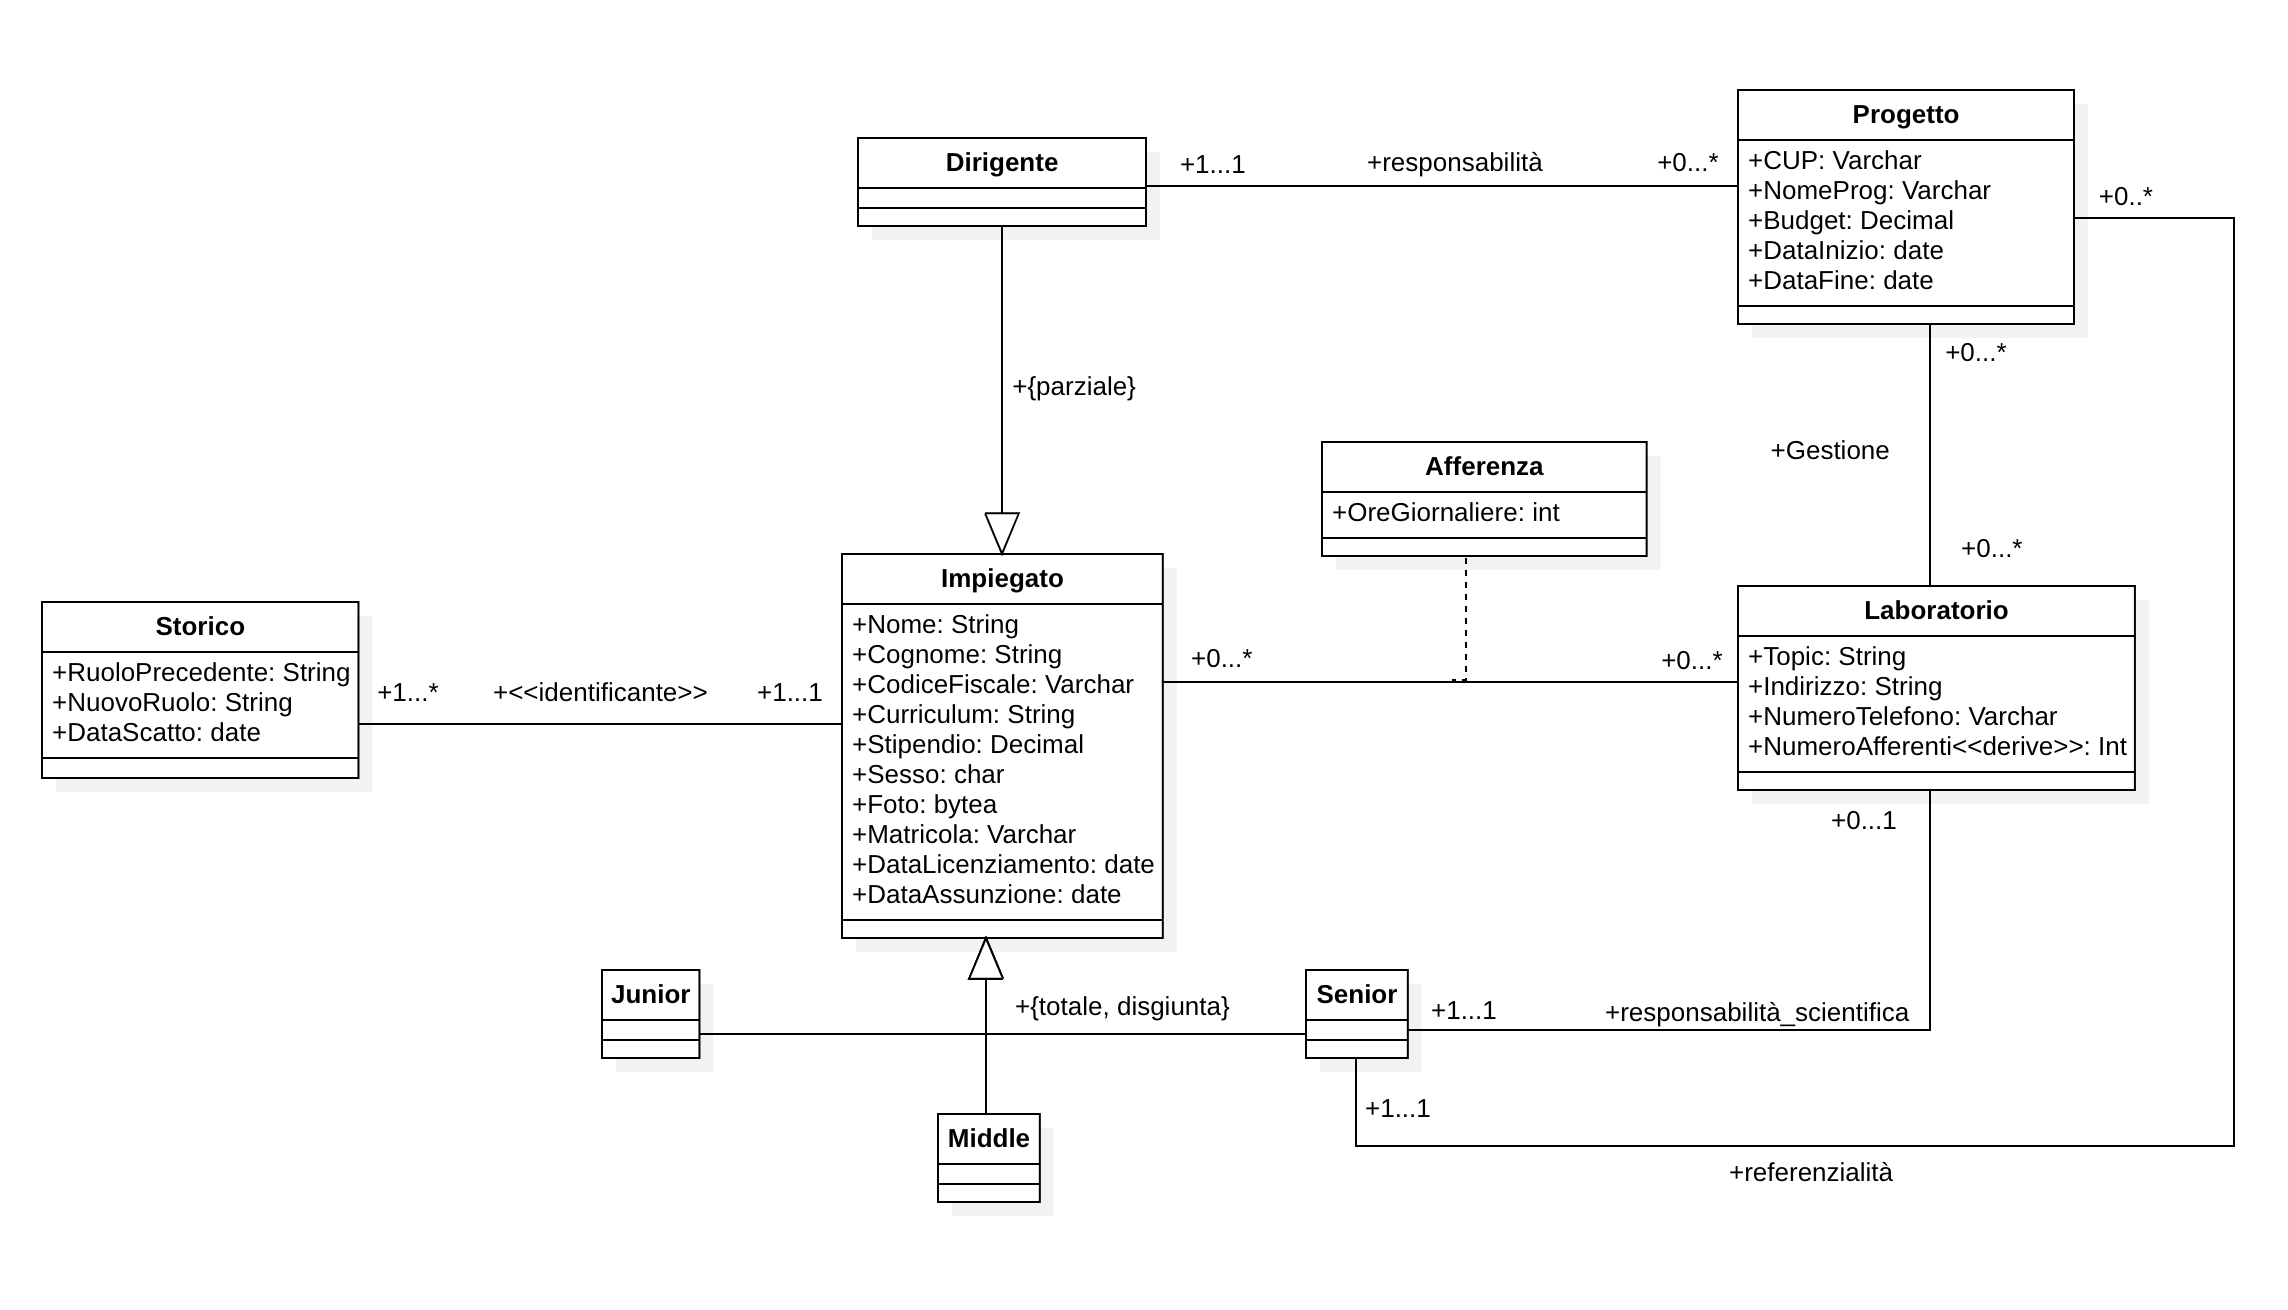
\includegraphics[width=\textwidth]{images/CONCETTUALE.png}
\end{figure}

\newpage

